\section{Исследование методов организации процесса обработки данных в КХЭД} \label{experiment}

Конфиденциальное хранилище электронных документов, как и любая другая система, может быть представлено в виде совокупности модулей, выполняющих различные функции. %Так как документооборот -- детерминированный процесс, каждый этап которого может быть детально расписан, можно рассматривать такие этапы в отдельности. 
Для каждого модуля можно определить варианты реализации, исходя из особенностей его работы. Наибольший интерес будут представлять следующие модули:
\begin{itemize}
	\item модуль обеспечения совместной работы пользователей;
	\item модуль хранения истории внесённых изменений;
	\item модуль обнаружения ошибок при обработке документа;
	\item модуль авторизации.
\end{itemize}
Остальные модули (передачи данных, разграничения доступа, защиты хранилища от несанкционированного доступа) реализуются стандартными методами и не представляют такого интереса.

\vspace{\baselineskip}
Для выбора реализации модулей КХЭД в соответствии с показателями эффективностями, которые будут описаны позднее, необходимо провести экспериментальное исследование существующих реализаций подобных модулей. Так как СЭД дороги и сложны в развёртывании, не все компании предоставляют демо-версии своих продуктов. Но и в случае наличия демо-версии довольно сложно её получить и оценить параметры (часто вместо демо-версии предоставляется презентация, отсутствует доступ к отдельным модулям системы). Существует и ещё один фактор, затрудняющий сложность проведения эксперимента: так как СЭД является системой массового обслуживания, для её объективного тестирования необходимо провести множество однотипных испытаний, включающих в себя работу нескольких испытуемых (пользователей СЭД) в течение длительного времени.

\vspace{\baselineskip}
С учётом всех вышеизложенных ограничений, было принято решение првоести имитационное моделирвоание модулей КХЭД в среде AnyLogic, приняв за описание моделей базовые принципы построения исследуемых модулей в различных реализациях.

\subsection{Модуль обеспечения совместной работы пользователей} \label{research_competition}

При совместной конкурентной работе пользователей в системе электронного документооборота существует проблема синхронизации вносимых изменений. Так, два редактора, работая над одним документом (но каждый со своим набором задач), во время внесения изменений блокируют работу друг друга, так как документ в рассматрвиаемом контексте -- ограниченный ресурс. Схема такой модели в среде AnyLogic представлена на рис. \ref{img:competition_old_scheme}.

\begin{figure}[h]
  \centering
  \includegraphics[width=1\textwidth]{competition_old_scheme}
  \caption{Схема конкурентной обработки документа с блокировкой}
  \label{img:competition_old_scheme}
\end{figure}

Здесь объекты $source$ моделируют источники заявок (по одной заявке в полчаса), $queue$ -- персональные очереди заявок на обработку, $hold$ -- элемент, блокирующий работу редактора (когда работает первый редактор, второй блокируется, и наоборот), $delay$ -- редакторы (время обработки заявки распределяется по нормальному закону со средним значением 25 минут, $\sigma=5$), $sink$ -- целевое хранилище, собирающее обработанные заявки.

\vspace{\baselineskip}
Альтернативой является такая схема организации обработки документов, при которой разрешено одновременное внесение изменений в документ, что справедливо для разрабатываемой системы. Это становится возможным благодаря регистрации не состояний документа, а вносимых в него изменений в виде разницы текущего и предыдущего состояний. Такая разностная запись называется <<патч>>. Пример патча см. на рис. \ref{img:git_patch}.

\begin{figure}[h]
  \centering
  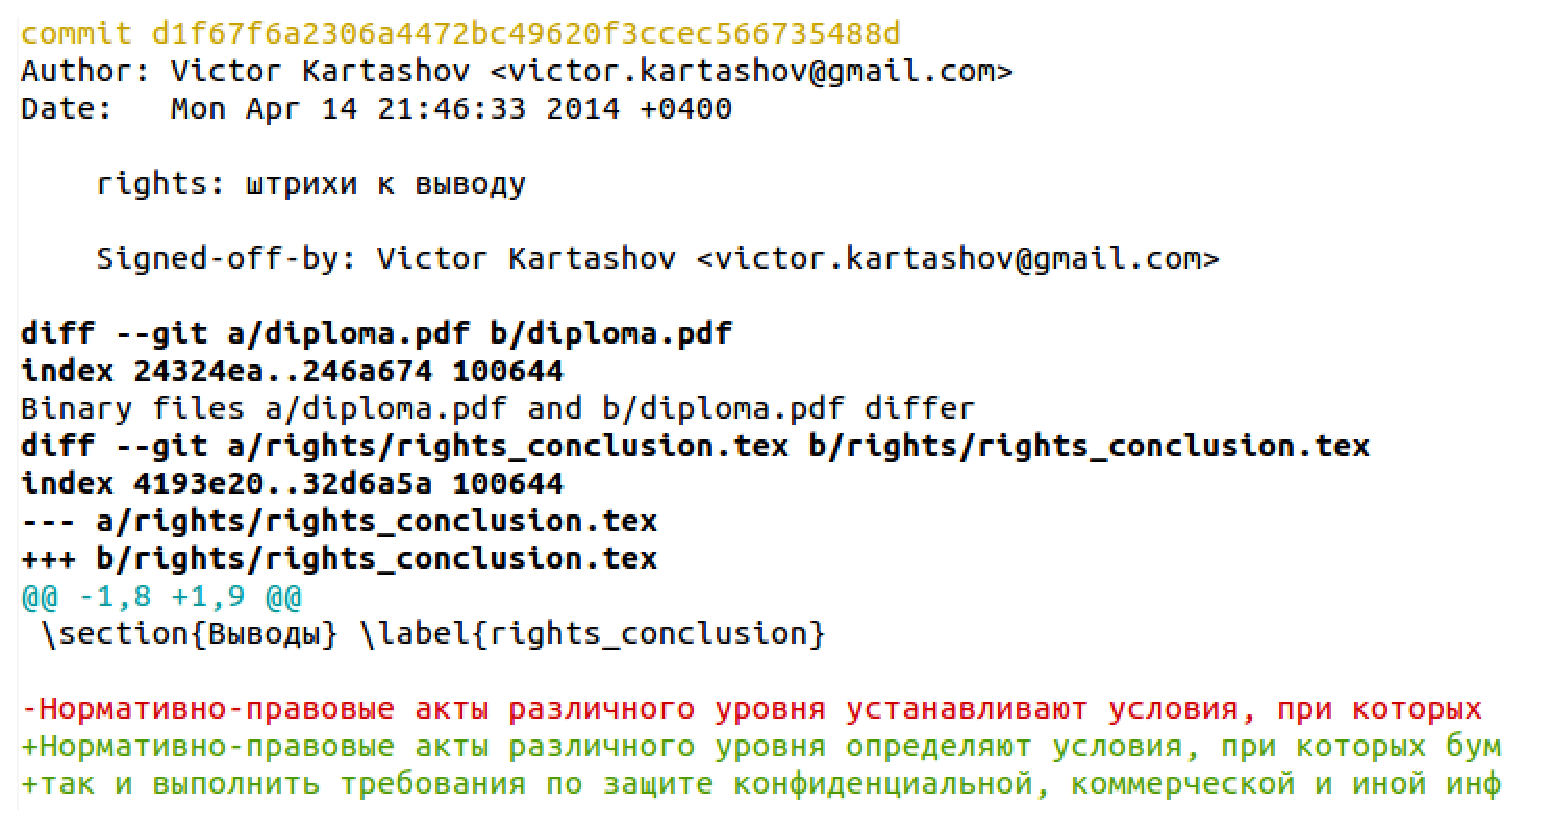
\includegraphics[width=1\textwidth]{git_patch}
  \caption{Пример записи состояния документа в виде патча}
  \label{img:git_patch}
\end{figure}

Данная реализация позволяет не только сократить объём хранимых данных, но и реализовать вышеописанную схему, ведь при таком подходе одновременное внесение изменений несколькими редакторами рассматривается не как изменение одного документа, а как создание набора новых записей. Результирующий документ получается путём последовательного применения таких патчей к исходному документу.

\vspace{\baselineskip}
Схема этой модели в среде AnyLogic представлена на рис. \ref{img:competition_new_scheme}.

\begin{figure}[h]
  \centering
  \includegraphics[width=1\textwidth]{competition_new_scheme}
  \caption{Схема конкурентной обработки документа без блокировки}
  \label{img:competition_new_scheme}
\end{figure}

\vspace{\baselineskip}
Элементы на этой схеме совпадают с элементами схемы рис. \ref{img:competition_old_scheme}, однако здесь отсутствуют блоки $hold$, а время обработки заявки распределяется по нормальному закону со средним значением 30 минут, $\sigma=6$ (из расчёта временного запаса на устранение ошибок слияния при одновременном переходе обработанных заявок в блок $sink$).

\vspace{\baselineskip}
В процессе эксперимента был промоделирован один рабочий день (с 9:00 до 18:00), в течение которого каждому из редакторов на обработку поступило 19 заявок. Число обработанных заявок в схеме с блокировкой показано на рис. \ref{img:competition_old_done}, в схеме без блокировок -- на рис. \ref{img:competition_new_done}.

\begin{figure}[h]
  \centering
  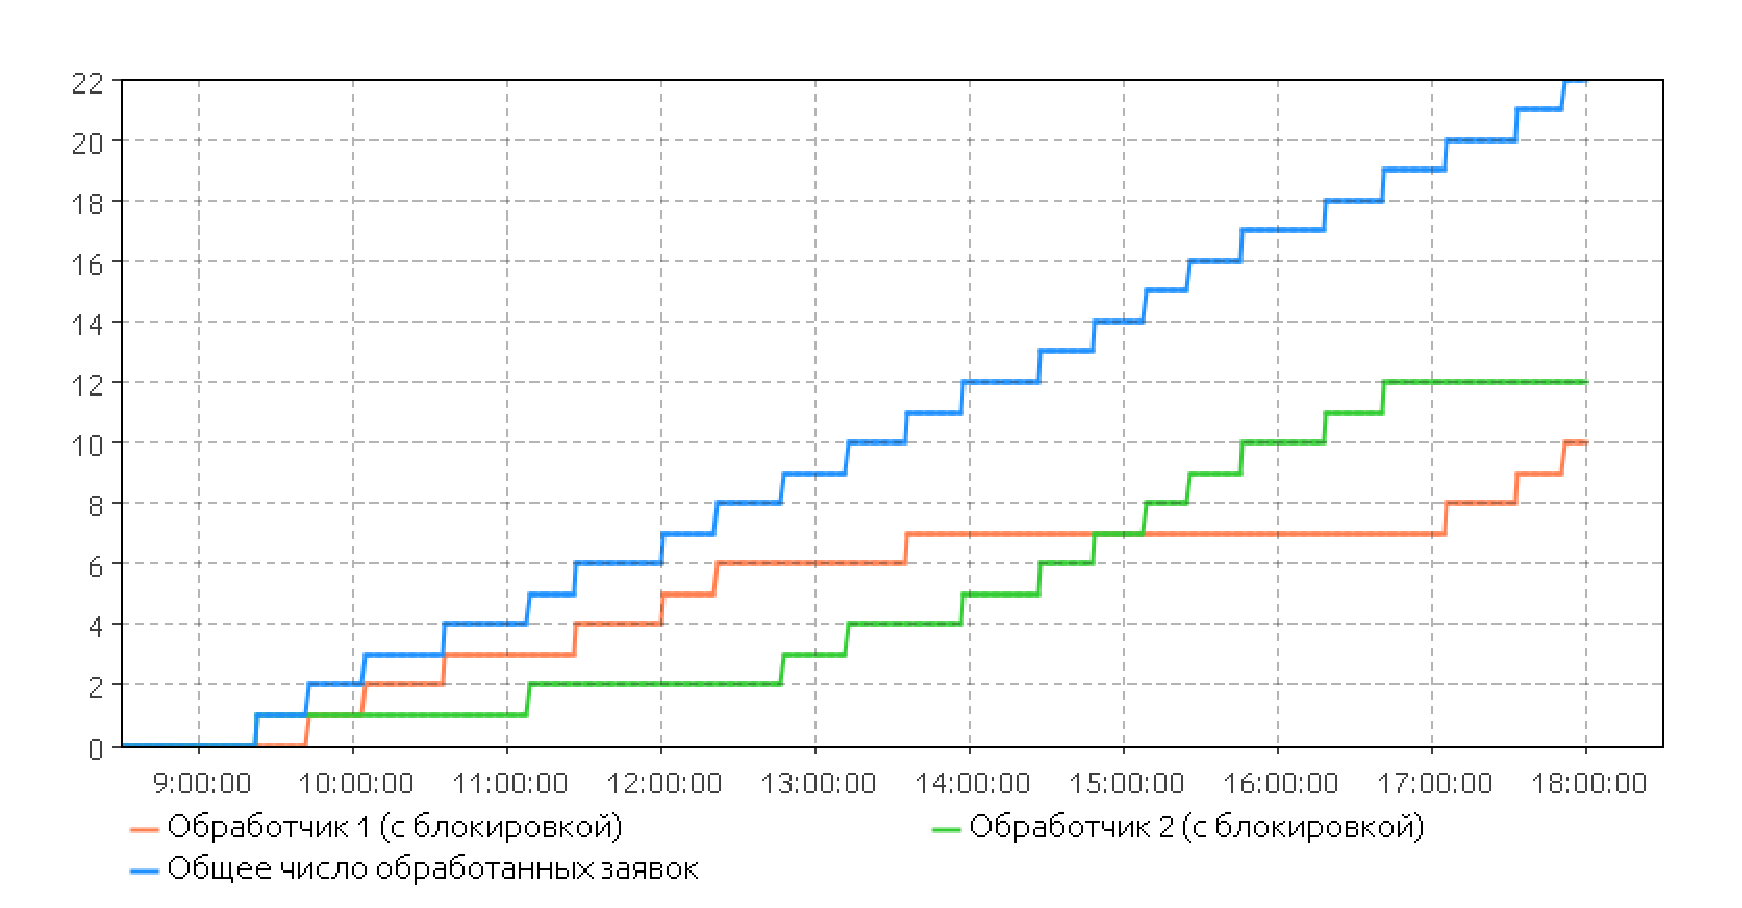
\includegraphics[width=1\textwidth]{competition_old_done}
  \caption{Число обработанных заявок в схеме с блокировкой}
  \label{img:competition_old_done}
\end{figure}

\begin{figure}[h]
  \centering
  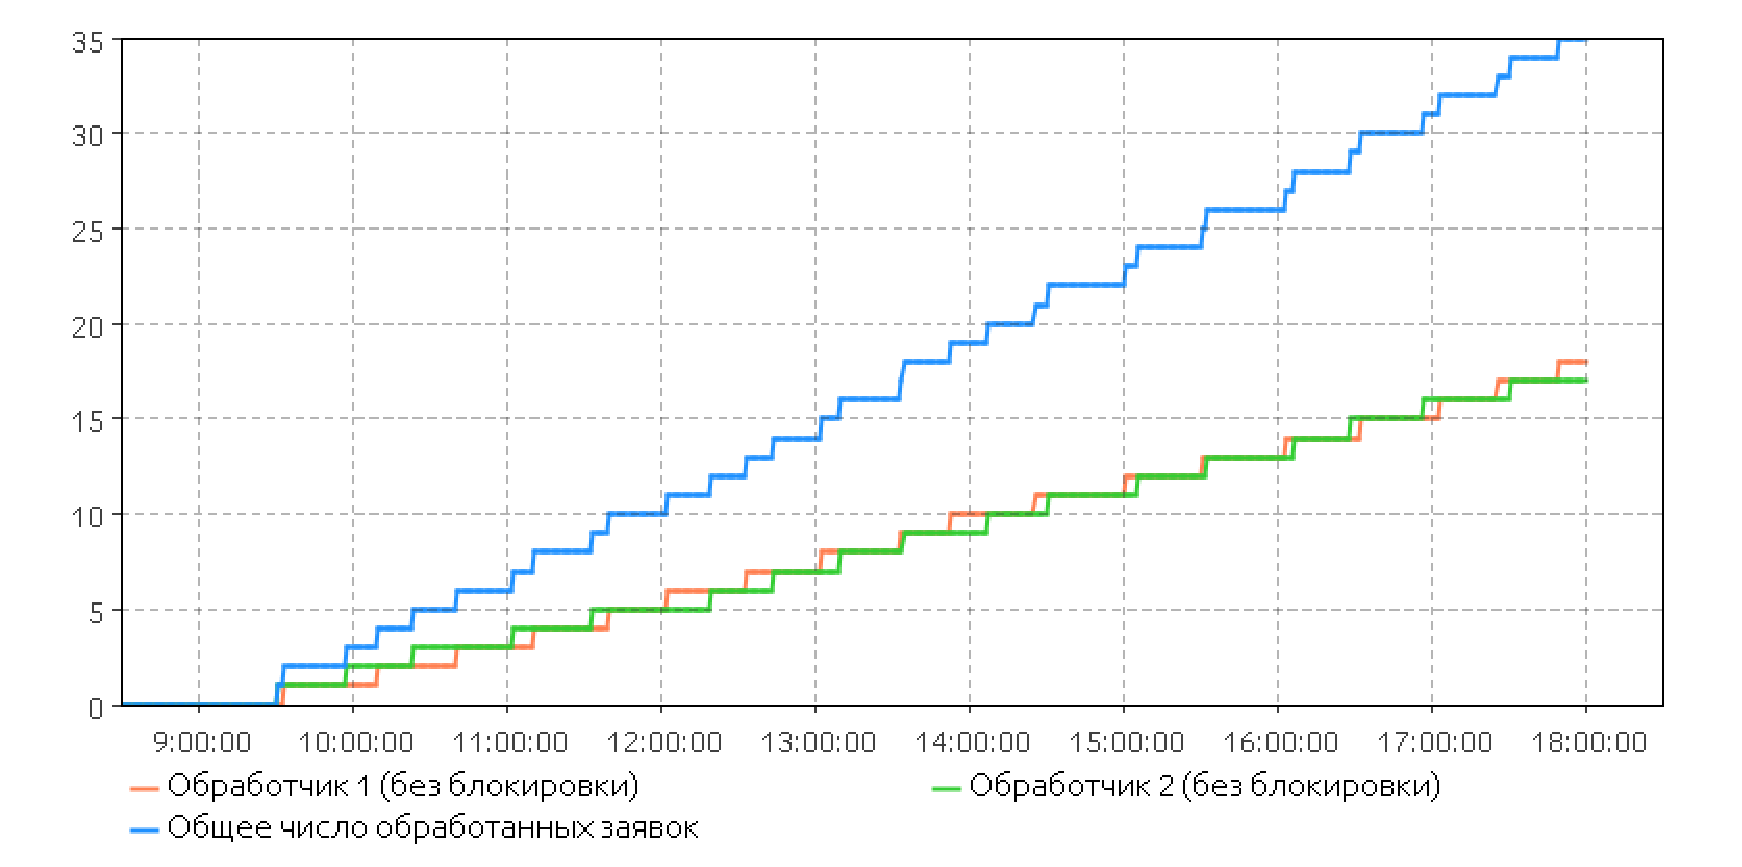
\includegraphics[width=1\textwidth]{competition_new_done}
  \caption{Число обработанных заявок в схеме без блокировки}
  \label{img:competition_new_done}
\end{figure}

\vspace{\baselineskip}
Как видно из представленных результатов, несмотря на б\textit{о}льшее среднее время обработки одной заявки, число успешно обработанных заявок в схеме без блокировки за один рабочий день в $~1.5$ раза больше, чем число успешно обработанных заявок в схеме с блокировкой за тот же период. Также по этим рисункам видно, что за счёт блокировок заявки редакторами в первой схеме обрабатывались неравномерно, в отличие от второй схемы. Дополнительным подтверждением этому служат временные диаграммы загруженности редакторов в течение рабочего дня, представленные на рис. \ref{img:competition_old_gantt} и \ref{img:competition_new_gantt}.

\begin{figure}[h]
  \centering
  \includegraphics[width=1\textwidth]{competition_old_gantt}
  \caption{Временная диаграмма загруженности редакторов в течение рабочего дня в схеме с блокировкой}
  \label{img:competition_old_gantt}
\end{figure}

\begin{figure}[h]
  \centering
  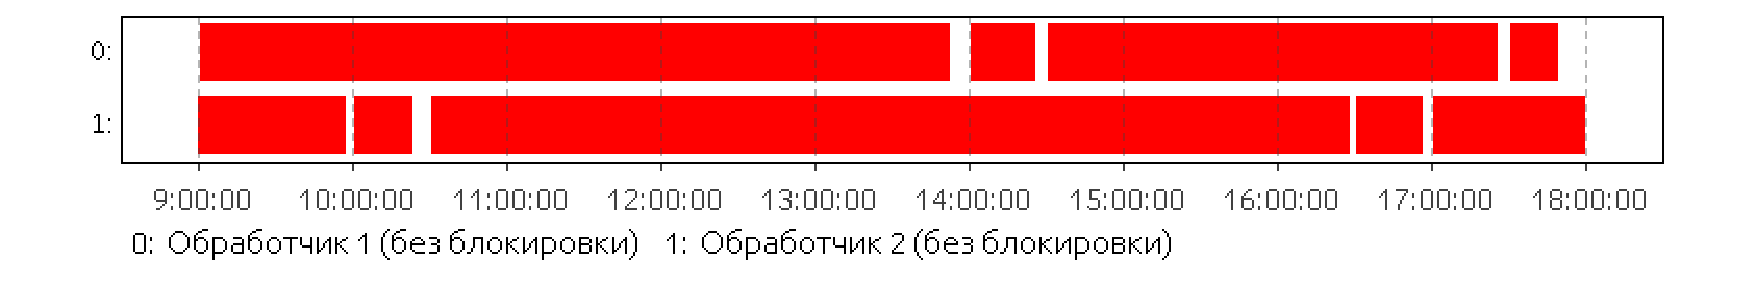
\includegraphics[width=1\textwidth]{competition_new_gantt}
  \caption{Временная диаграмма загруженности редакторов в течение рабочего дня в схеме без блокировки}
  \label{img:competition_new_gantt}
\end{figure}

\vspace{\baselineskip}
Эти рисунки наглядно показывают время бездействия редакторов в схеме с блокировкой (два редактора работают с загрузкой, равной 100\% загрузке одного редактора). Такого продолжительного простоя можно избежать только обрабатывая параллельно несколько документов так, чтобы время блокировок сводилось к минимуму. Таким образом, появляется дополнительная задача временн\textit{о}го планирования. При этом схема без блокировок помогает эффективно использовать рабочее время без дополнительного планирования.

\vspace{\baselineskip}
Ещё один немаловажный показатель -- загруженность очереди на обработку. Соответствующие графики приведены на рис. \ref{img:competition_old_queue} и \ref{img:competition_new_queue}.

\begin{figure}[h]
  \centering
  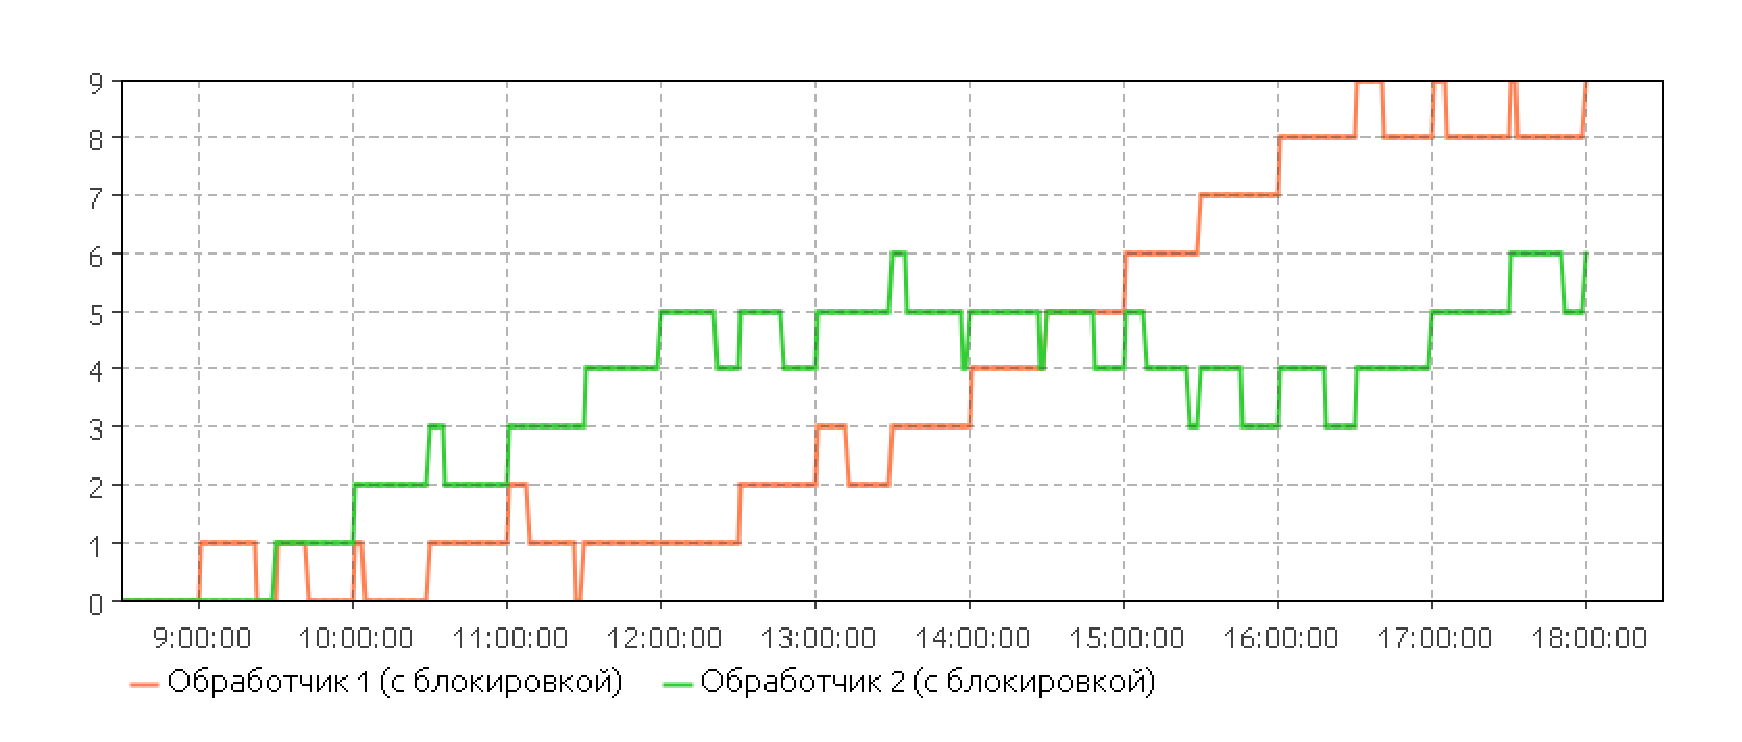
\includegraphics[width=1\textwidth]{competition_old_queue}
  \caption{Загруженность очереди на обработку в схеме с блокировкой}
  \label{img:competition_old_queue}
\end{figure}

\begin{figure}[h]
  \centering
  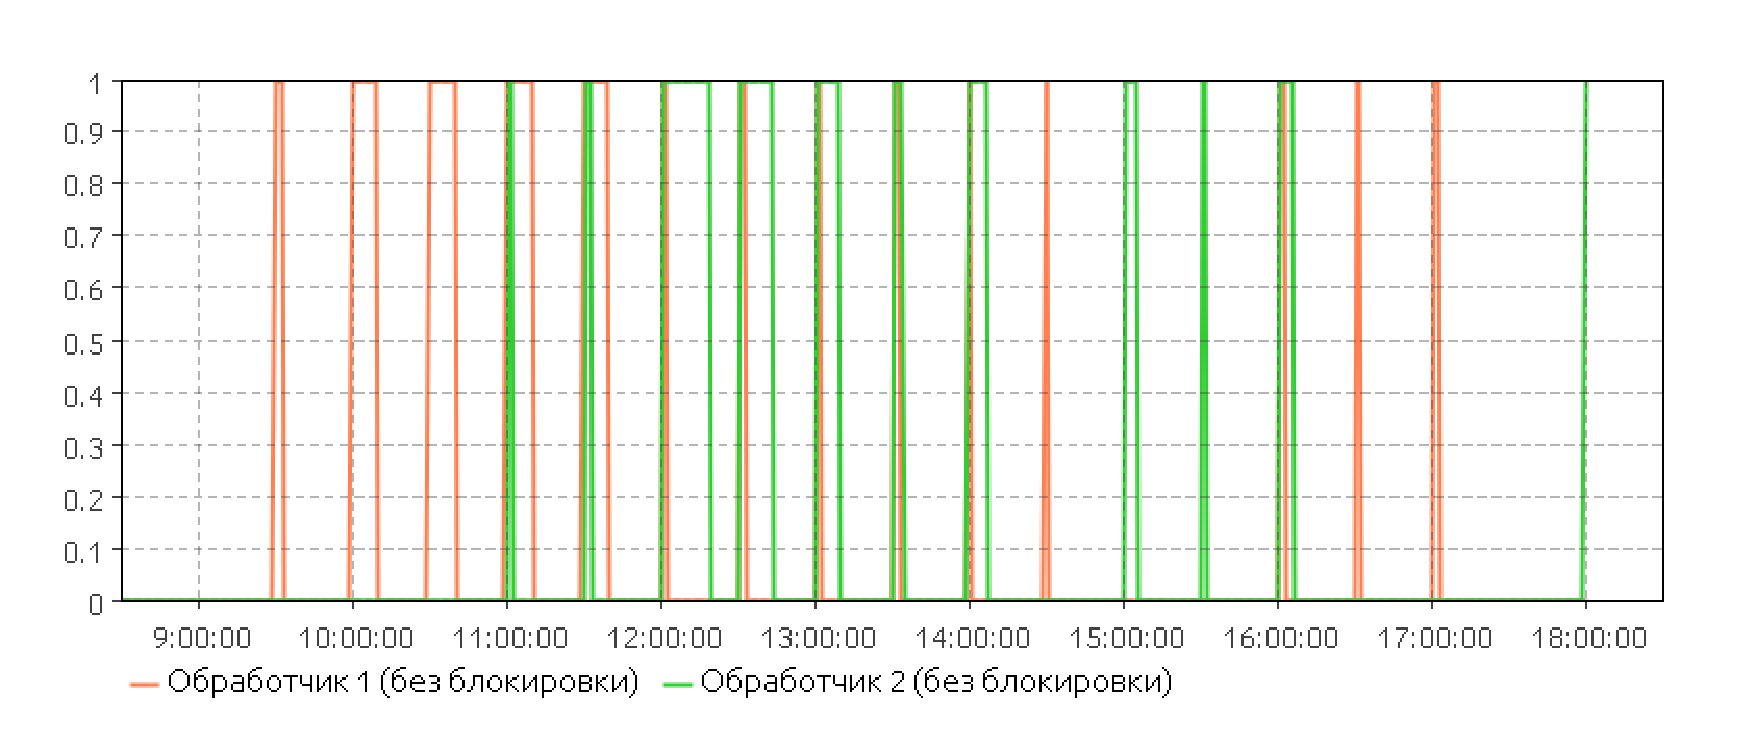
\includegraphics[width=1\textwidth]{competition_new_queue}
  \caption{Загруженность очереди на обработку в схеме без блокировки}
  \label{img:competition_new_queue}
\end{figure}

\vspace{\baselineskip}
Как видно, при использовании схемы с блокировкой заполняемость очереди имеет тенденцию к росту, что в конечном итоге приведёт к ситуации, в которой заявки одного конкретного редактора будут полностью удовлетворены только по завершении работ остальными редакторами. В то же время, очереди в схеме без блокировок не имеют подобной тенденции, и заявки, находящиеся в них, своевременно удовлетворяются.

\vspace{\baselineskip}
Таким образом, при совместной работе пользователей над одним документом в системе электронного документооборота целесообразно использовать предложенную схему организации процесса без блокировок.			% Конкурентная обработка документа
\subsection{Модуль обнаружения ошибок при обработке документа} \label{research_feedback}

При обработке документов автоматиизирвоанным способом существует возможность обнаружения ошибок на стадии редактирования, т.е. до отправки документа далее по цепочке обработки. В таком случае ошибка либо устраняется автоматически, либо создаётся новая задача на устранение ошибки тому же редактору, который эту ошибку допустил.

\vspace{\baselineskip}
Одной из разновидностей ошибки такого рода является некорректное обращение к полям документа. Стоит отметить, что речь здесь идёт не о метаданных, сопровождающих документ, а об информации, содержащейся непосредственно в документе. Например, для совместной работы, описанной в гл. \ref{research_competition}, таким обращением будет считаться попытка редактирвоания полей документа, обработкой которых уже занимается другой редактор.

\vspace{\baselineskip}
Для эксперимента были рассмотрены две схемы: одна --- <<классическая>>, без обнаружения ошибок такого рода (многие СЭД не предоставляют подобного сервиса, регулируя только поля метаданных, см. табл. \ref{table:products}), другая --- согласно описанной выше схеме, реализованная в описываемой разработке.

\vspace{\baselineskip}
На рис. \ref{img:feedback_old_scheme} представлена схема без автоматизированного обнаружения ошибок. Возврат на доработку при такой организации возможен, но осуществляется в ручном режиме: редактор, получивший на вход задания документ с ошибкой, отправляет его на переработку предыдущему редактору (в реальной системе он будет передавать документ соседнему звену в обратном направлении, однако как показывает практика, в случае подчинения низших звеньев высшим документ будет возвращаться до первого редактора). Последний редактор в случае допуска ошибки получит неверный документ, на схеме приёмник таких результатов обозначен $sink$. Корректно обработанные заявки приходит в пункт $sink2$. Разветвления после обработчиков работают по вероятностному принципу с вероятностью обнаружения ошибки $P_{txt}'$.
 
\begin{figure}[h!]
  \centering
  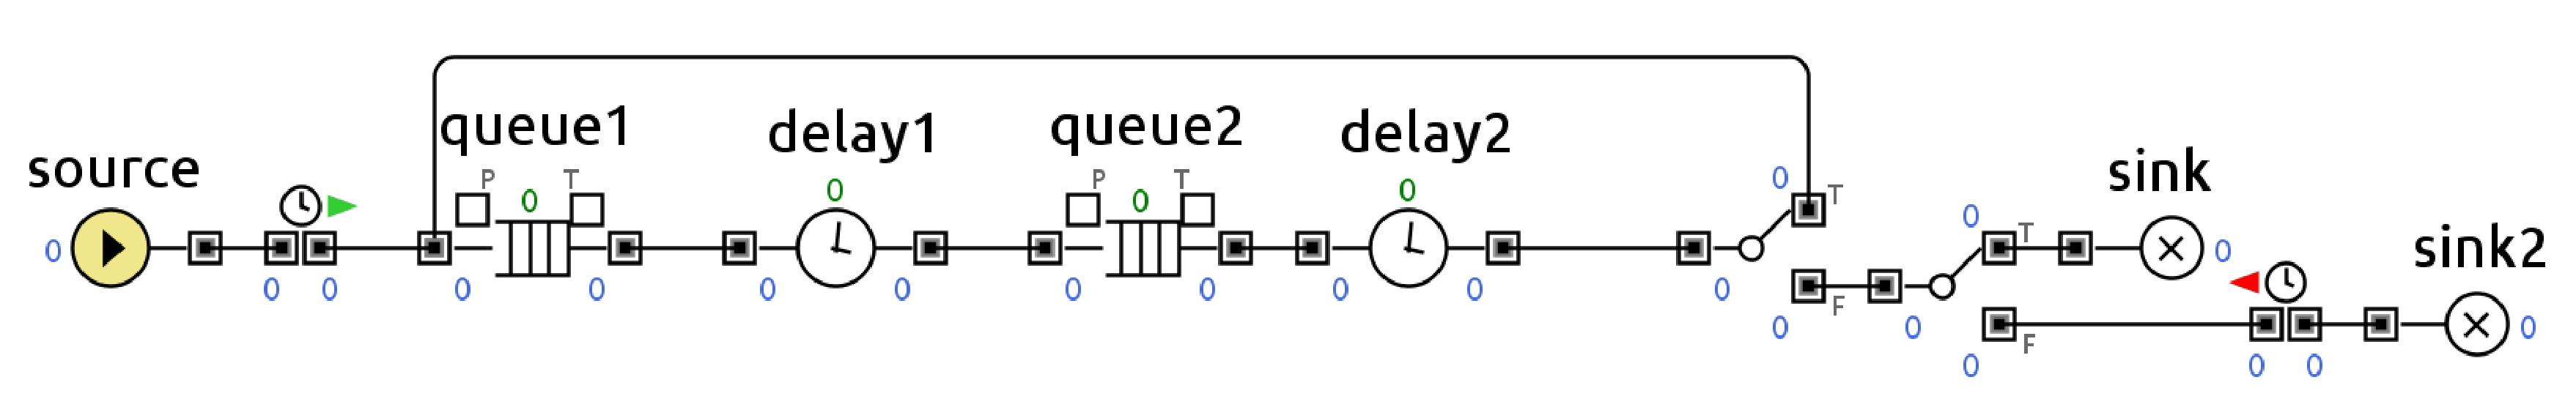
\includegraphics[width=1\textwidth]{feedback_old_scheme}
  \caption{Схема коррекции ошибок ручным методом}
  \label{img:feedback_old_scheme}
\end{figure}

\vspace{\baselineskip}
В случае автомтизированного обнаружения ошибок (рис. \ref{img:feedback_new_scheme}) задание на переработку генерируется автоматически для того редактора, который допустил ошибку. Таким образом, даже последний редактор в цепочке имеет возможность исправить допущенную ошибку перед публикацией документа.

\begin{figure}[h!]
  \centering
  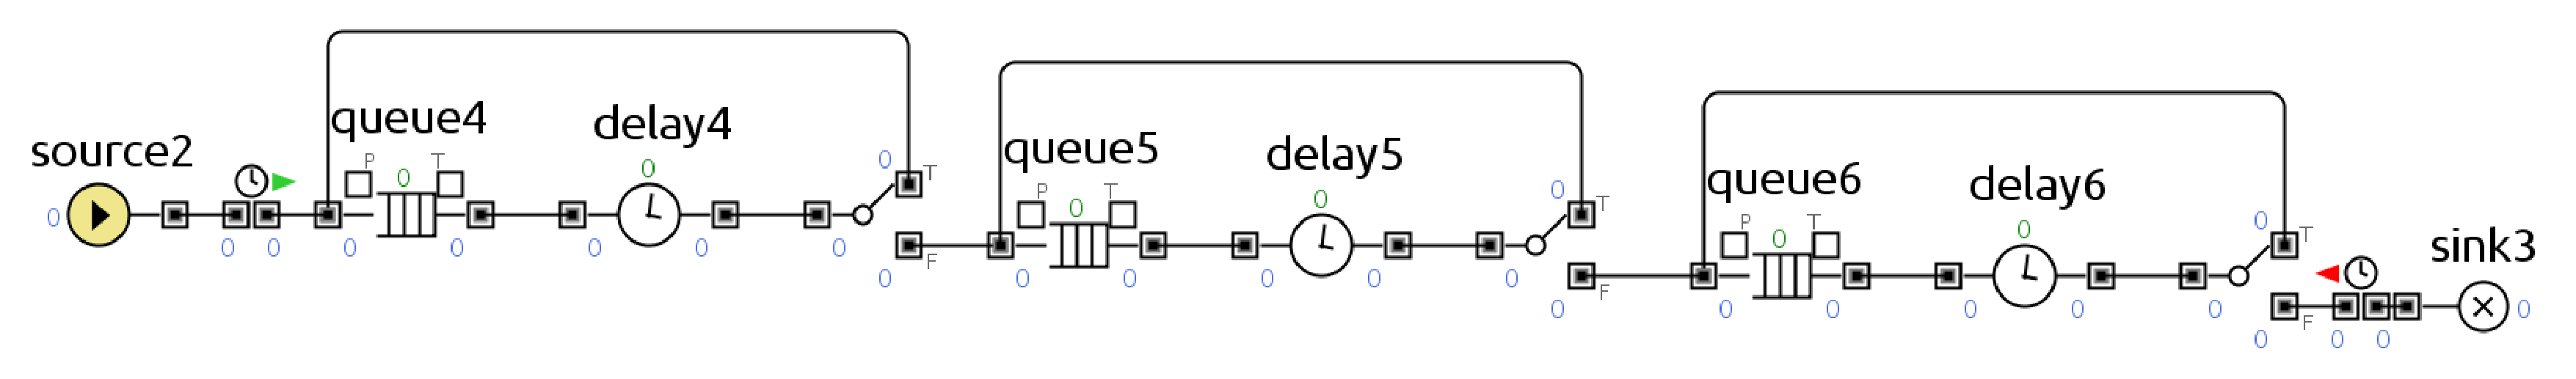
\includegraphics[width=1\textwidth]{feedback_new_scheme}
  \caption{Схема коррекции ошибок автоматизированным методом}
  \label{img:feedback_new_scheme}
\end{figure}

\vspace{\baselineskip}
Одним из показателей эффективности метода организации процесса обработки документов является число корректно обработанных заявок. Как и в случае совместной работы пользователей, заявки генерируются по одной за полчаса реального времени, моделируется один рабочий день (с 9:00 до 18:00). Параметры обработчиков совпадают с описанными в гл. \ref{research_competition}. Результат моделирования представлен на рис. \ref{img:feedback_done}.

\begin{figure}[h!]
  \centering
  \includegraphics[width=1\textwidth]{feedback_done}
  \caption{Число обработанных заявок в схемах с обратной связью}
  \label{img:feedback_done}
\end{figure}

\vspace{\baselineskip}
Как видно из рисунка, схема с автоматизирвоанным обнаружением ошибок позволяет обработать больше заявок за ограниченный промежуток времени. Также можно заметить, что частота, с которой заявкам присваивался статус <<корректно обработанная>>, выше в схеме с АС. Это позволяет предположить, что среднее время обработки одной заявки при такой организации меньше, чем при ручном обнаружении ошибок. Данная гипотеза подтверждается графиком, приведённым на рис. \ref{img:feedback_mean}.

\begin{figure}[h!]
  \centering
  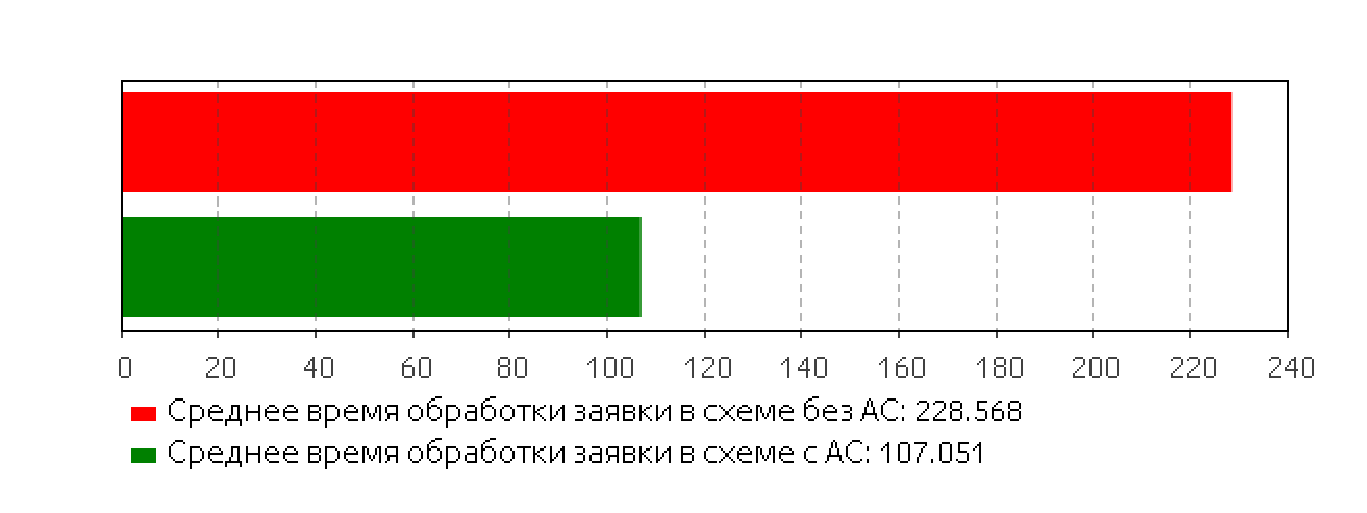
\includegraphics[width=1\textwidth]{feedback_mean}
  \caption{Среднее время обработки одной заявки в схемах с обратной связью}
  \label{img:feedback_mean}
\end{figure}

\vspace{\baselineskip}
Уменьшение времени обработки заявки происходит за счёт того, что в случае необходимости исправления ошибки над документом работает один редактор из цепочки (тот, который допустил ошибку), а не все. Более того, среднее время обработки заявки в схеме без АС можно считать заниженным, т.к. в нём не учтено время поиска ошибки, а сама вероятность её обнаружения оценена довольно высоко --- наравне с АС. 

\vspace{\baselineskip}
Таким образом, для снижения времени обработки заявок целесообразно использовать систему автоматического обнаружения ошибок.				% Возврат на доработку